\section{Différents types de rupture}

Ce projet a pour but de détecter les différents types de rupture listés ci-dessous :

\begin{itemize}
	\item Changement d'image;
	\item Fondu d'image.
\end{itemize}

\subsection{Changement d’image}
Un changement d’image est construit de deux images qui viennent de deux scènes différents, sans fusion entre ces deux scènes :

\begin{figure}[h!]
   \begin{minipage}[c]{.46\linewidth}
	  \centering
      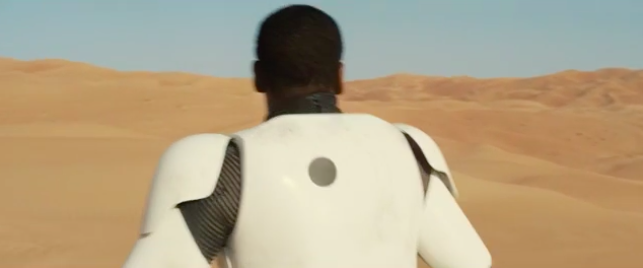
\includegraphics[scale=0.3]{images/rupture1-1.png}
      \caption{\label{Avant} Image avant la rupture}
   \end{minipage} \hfill
   \begin{minipage}[c]{.46\linewidth}
      \centering
      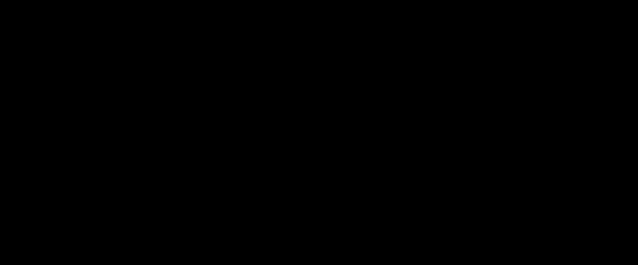
\includegraphics[scale=0.3]{images/rupture1-2.png}
      \caption{\label{Après} Image après la rupture}
   \end{minipage}
\end{figure}


\subsection{Fondu d'image}
Un fondu d’image est construit de deux images qui viennent de deux scènes différents, mais il y a de fusion entre ces deux scènes :

\begin{figure}[h!]
   \begin{minipage}[c]{.46\linewidth}
	  \centering
      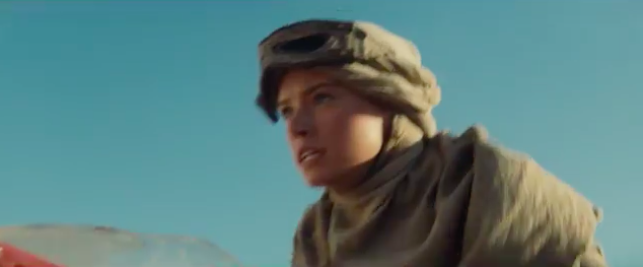
\includegraphics[scale=0.3]{images/rupture2-1.png}
      \caption{\label{Avant} Image avant la rupture}
   \end{minipage} \hfill
   \begin{minipage}[c]{.46\linewidth}
      \centering
      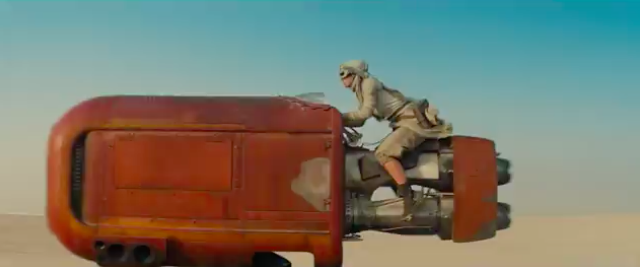
\includegraphics[scale=0.3]{images/rupture2-2.png}
      \caption{\label{Après} Image après la rupture}
   \end{minipage}
\end{figure}